\scanpage{25}
Théorème : supposons qu'il n'existe pas deux sommets tels que tte ps. droite passe par l'un d'eux, i.e. qu'on ne soit pas dans l'un des cas $\mathrm I_N$, $\mathrm I_{p,q}$, $\mathrm{II}_{pq}$. Supposons de plus \deleted{$N\geq5$ (sinon c'est le cas $\mathrm{II}_{4}$)} \deleted{et} que $K$ ne contienne pas de sous-arrangement du type $\mathrm{II}_5$, elle est de l'un des types suivants : \deleted{$\unsure{\mathrm{III}_{4}|\mathrm{II}_{4}}$}

\margin{$4+3=7$ sommets}
$\mathrm{III}_{6})$ \unsure{Arrangement} \unsure{tétraédral|tétraédrale}
\figure{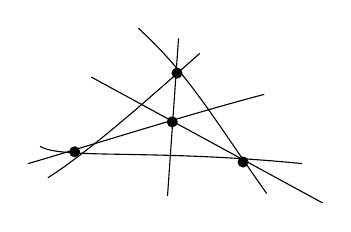
\begin{tikzpicture}[x=.010cm,y=-.010cm]
\draw (25,195) .. controls (80,160) and (157,91) .. (218,37);
\draw (0,177) .. controls (82,153) and (198,116) .. (300,89);
\draw (15,155) .. controls (42,172) and (155,158) .. (348,177);
\draw (80,67) -- (374,227);
\draw (140,5) .. controls (205,65) and (231,113) .. (303,215);
\draw (191,18) -- (177,218);
\foreach \x/\y in {59/162,183/124,189/62,273/175}{\fill (\x,\y) circle[radius=2pt];}
\end{tikzpicture}}

\margin{$6+3=9$ sommets}
$\mathrm{IV}_{7})$ Arrangement d'un quadrilatère et de ses trois diagonales
\figure{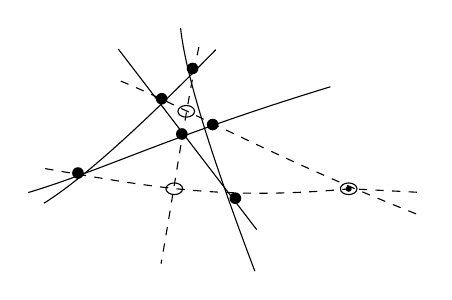
\begin{tikzpicture}[x=.008cm,y=-.008cm]
\draw (25,255) .. controls (87,216) and (181,131) .. (298,11);
\draw (0,238) .. controls (120,202) and (224,148) .. (480,70);
\draw (143,10) -- (363,297);
\draw (242,-23) .. controls (248,30) and (270,125) .. (360,363);
\draw[dashed] (147,61) .. controls (250,103) and (386,181) .. (624,275);
\draw[dashed] (27,200) .. controls (196,229) and (307,251) .. (511,232) -- (627,238);
\draw[dashed] (271,7) .. controls (250,106) and (233,226) .. (211,351);
\foreach \x/\y in {79/207,212/89,261/41,244/145,293/130,329/247}{\fill (\x,\y) circle[radius=2.1pt];}
\foreach \x/\y in {251/109,232/232,509/232}{\draw (\x,\y) ellipse[x radius=3pt,y radius=2.1pt];}
\fill (509,232) circle[radius=1.1pt];
\end{tikzpicture}}

\uline{NB} $\mathrm{III}_{6}$ et $\mathrm{IV}_{7}$ sont \inserted{avec $\mathrm I_{2,2}$ (\unsure{quadri avec|quadr. avec|quadrilatère avec} $1$ diagonale) et $\mathrm I_N$ $(N\geq5)$} les \deleted{configurations} \inserted{\unsure{arrangmts}} avec $N\geq5$ qui ne contiennent pas l'arrangement $\mathrm I'_{3,2}$ ni $\mathrm{II}_5$. Tout \unsure{arrangmt|arrangement} sans bigone, \deleted{contient types et \unsure{qui n'est}} est soit du type $\mathrm{II}_4$, soit contient un des types $\boxed{\mathrm I'_{32},\mathrm{II}_5,\mathrm{III}_6}$ (et s'il ne contient $\mathrm I'_{3,2}$ ni $\mathrm{II}_5$, c'est un type $\mathrm{III}_6$ ou $\mathrm{IV}_7$). Ces trois types \deleted{sont} ``latticiels''\,; i.e. dans le cas 2-dimensionnel, les \unsure{facettes|faces} fermées forment un lattice : \deleted{\unsure{deux}} l'intersection de deux faces fermées non vides est une facette.
% archive sheet number: 24
